

\documentclass[aspectratio=169]{beamer}\usepackage[]{graphicx}\usepackage[]{color}
%% maxwidth is the original width if it is less than linewidth
%% otherwise use linewidth (to make sure the graphics do not exceed the margin)
\makeatletter
\def\maxwidth{ %
  \ifdim\Gin@nat@width>\linewidth
    \linewidth
  \else
    \Gin@nat@width
  \fi
}
\makeatother

\definecolor{fgcolor}{rgb}{0.345, 0.345, 0.345}
\newcommand{\hlnum}[1]{\textcolor[rgb]{0.686,0.059,0.569}{#1}}%
\newcommand{\hlstr}[1]{\textcolor[rgb]{0.192,0.494,0.8}{#1}}%
\newcommand{\hlcom}[1]{\textcolor[rgb]{0.678,0.584,0.686}{\textit{#1}}}%
\newcommand{\hlopt}[1]{\textcolor[rgb]{0,0,0}{#1}}%
\newcommand{\hlstd}[1]{\textcolor[rgb]{0.345,0.345,0.345}{#1}}%
\newcommand{\hlkwa}[1]{\textcolor[rgb]{0.161,0.373,0.58}{\textbf{#1}}}%
\newcommand{\hlkwb}[1]{\textcolor[rgb]{0.69,0.353,0.396}{#1}}%
\newcommand{\hlkwc}[1]{\textcolor[rgb]{0.333,0.667,0.333}{#1}}%
\newcommand{\hlkwd}[1]{\textcolor[rgb]{0.737,0.353,0.396}{\textbf{#1}}}%
\let\hlipl\hlkwb

\usepackage{framed}
\makeatletter
\newenvironment{kframe}{%
 \def\at@end@of@kframe{}%
 \ifinner\ifhmode%
  \def\at@end@of@kframe{\end{minipage}}%
  \begin{minipage}{\columnwidth}%
 \fi\fi%
 \def\FrameCommand##1{\hskip\@totalleftmargin \hskip-\fboxsep
 \colorbox{shadecolor}{##1}\hskip-\fboxsep
     % There is no \\@totalrightmargin, so:
     \hskip-\linewidth \hskip-\@totalleftmargin \hskip\columnwidth}%
 \MakeFramed {\advance\hsize-\width
   \@totalleftmargin\z@ \linewidth\hsize
   \@setminipage}}%
 {\par\unskip\endMakeFramed%
 \at@end@of@kframe}
\makeatother

\definecolor{shadecolor}{rgb}{.97, .97, .97}
\definecolor{messagecolor}{rgb}{0, 0, 0}
\definecolor{warningcolor}{rgb}{1, 0, 1}
\definecolor{errorcolor}{rgb}{1, 0, 0}
\newenvironment{knitrout}{}{} % an empty environment to be redefined in TeX

\usepackage{alltt} % comment out for handouts

\usepackage{graphicx}
\usepackage{color}
\usepackage[version = 3]{mhchem}

\usepackage{pgfpages}
% Note: going to 2 up seems to deactivate certain hyperlinks, like those in lists
%\pgfpagesuselayout{2 on 1}[letterpaper, border shrink = 5 mm] % uncomment for handouts

\usepackage{remreset}% tiny package containing just the \@removefromreset command
\makeatletter
\@removefromreset{subsection}{section}
\makeatother
\setcounter{subsection}{1}

\usepackage{multicol}

\usetheme{Singapore} % comment out for totally plain look; Singapore is still quite simple
% note that Singapore cannot do any kind of frames, rounded boxes etc
\setbeamertemplate{blocks}[rounded][shadow=true]
\setbeamertemplate{navigation symbols}{} % cancels lower navigation symbols

\graphicspath{{./graphics/}}
\logo{
\includegraphics[height = 0.75 cm]{DPU_Logo_2011b.pdf}}

\title{Using \texttt{R} to Make Sense of NMR Datasets}
\author{Prof. Bryan Hanson Dept. of Chemistry \& Biochemistry DePauw University}
\date{\today}
\IfFileExists{upquote.sty}{\usepackage{upquote}}{}
\begin{document}



\section*{What is \texttt{R}?}

\begin{frame}{Using \texttt{R} to Make Sense of NMR Datasets}
\begin{center}
Prof. Bryan A. Hanson\\
Dept. of Chemistry \& Biochemistry\\
DePauw University, Greencastle Indiana\\

\begin{center}
  
\includegraphics[scale = 0.6]{PANIClogo.jpg}
\end{center}

Presentation available at \href{https://github.com/bryanhanson/PANIC2017}{\textcolor{red}{github.com/bryanhanson/PANIC2017}}\\
Additional references \& resources on last slide
\end{center}
\end{frame}


%%%%%

\begin{frame}{What Exactly is \texttt{R}?}
  \begin{itemize}
    \item \texttt{R} is a free software "environment" for statistical computing and graphics
    \item The Ecosystem:
      \begin{itemize}
        \item Base \texttt{R} via "R-Core"
        \item Add-on packages from many authors
          \begin{itemize}
            \item Comprehensive \texttt{R} Archival Network (aka CRAN) ($>$10,000 packages)
            \item Bioconductor ($>$1,300 packages)
            \item Unofficial repositories: Github, Gitlab, SourceForge etc.
          \end{itemize}
        \item Support forums
        \item User guides galore!
      \end{itemize}
  \end{itemize}
\end{frame}

%%%%%

\begin{frame}{The Ecosystem: Support Resources}
  \begin{itemize}
    \item \href{https://cran.r-project.org/manuals.html}{\textcolor{red}{Official Documentation}}
    \item \href{https://cran.r-project.org/web/views/}{\textcolor{red}{Focused, Topical Task Views}}
    \item \href{https://www.r-bloggers.com/}{\textcolor{red}{\texttt{R}-Bloggers}}: over 600 \texttt{R}-oriented bloggers
    \item \href{https://stackoverflow.com/questions/tagged/r}{\textcolor{red}{Stack Overflow}}: over 160K questions on use of \texttt{R}
    \item \href{https://stackoverflow.com/tags/r/info}{\textcolor{red}{Hundreds}} of "Intro to \texttt{R}" documents on the web
    \item \href{https://stackoverflow.com/tags/r/info}{\textcolor{red}{Dozens}} of free \texttt{R} books on the web
    \item Many packages have a "vignette" or user guide.
    \item More resources on last slide.
  \end{itemize}
\end{frame}

%%%%%

\begin{frame}{Features of \texttt{R}}
  \begin{itemize}
    \item Written by statisticians
    \item " \ldots a rather unlikely linguistic cocktail \ldots"\footnote{\href{http://r.cs.purdue.edu/pub/ecoop12.pdf}{\textcolor{red}{Structure of the R Language}}}
    \item Cross-Platform: Windows, Linux, Mac OS
    \item Infrastructure:  ready integration, interactive options
    \item Interfaces to many other languages, programs
      \begin{itemize}
        \item SAS, SPSS, python, JavaScript, MATLAB, C++ etc.
      \end{itemize}
    \item Several ways of running in parallel, using multiple cores
    \item Command line, or several GUI options
  \end{itemize}

\end{frame}

%%%%%

\begin{frame}{\texttt{R} is Open Source}
  \begin{itemize}
    \item Free!
    \item Transparent: All code readily available for inspection
    \item "Given enough eyeballs, all bugs are shallow" -- Linus Torvalds
    \item Many parts of the ecosystem are community driven
  \end{itemize}

\begin{quote}
\begin{center}
\begin{Large}
"Open source means everyone can see my stupid mistakes.\\
Version control means everyone can see every stupid mistake I've ever made."
\end{Large}
\end{center}
\end{quote}

\begin{flushright}
\href{https://kbroman.wordpress.com/2011/08/17/the-stupidest-r-code-ever/}{\textcolor{red}{Karl Broman}}
\end{flushright}

\end{frame}

%%%%%

\begin{frame}{Do People Use \texttt{R}?\footnote{\href{r4stats.com/articles/popularity/}{Bob Muenchen r4stats.com/articles/popularity/}}}
\begin{center}
  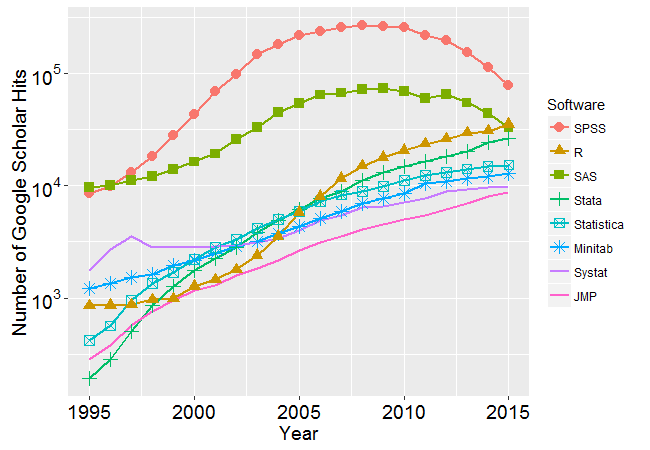
\includegraphics[scale = 0.4]{w1408b.png}
\end{center}
\end{frame}

%%%%%

\begin{frame}{Who Uses \texttt{R}?}
\begin{multicols}{2}
  \begin{itemize}
    \item AirBnB
    \item Zillow\footnote{\href{http://www.slideshare.net/NicholasMcClure1/python-datascienceatzillow}{\textcolor{red}{Data Science at Zillow}}}
    \item Etsy
    \item NYT
    \item Twitter
    \item Facebook
  \end{itemize}
\columnbreak
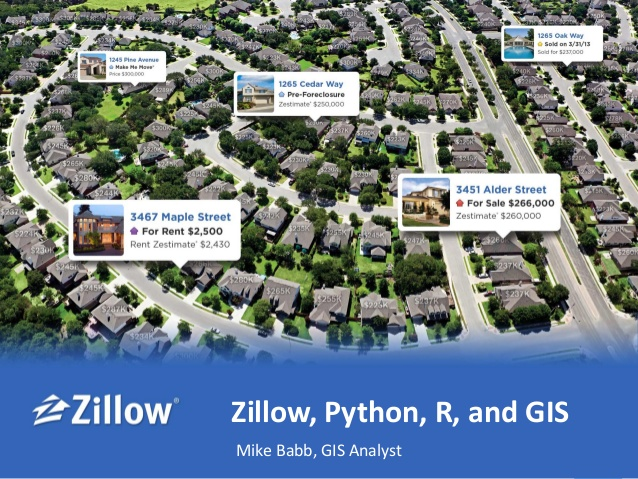
\includegraphics[scale = 0.25]{data-science-at-zillow-29-638.jpg}
\end{multicols}

\end{frame}

%%%%%

\begin{frame}{User Contributed Packages\footnote{\href{gist.github.com/daroczig/}{\textcolor{red}{Script} by Gergely Dar\'{o}czi}}}
\begin{center}
  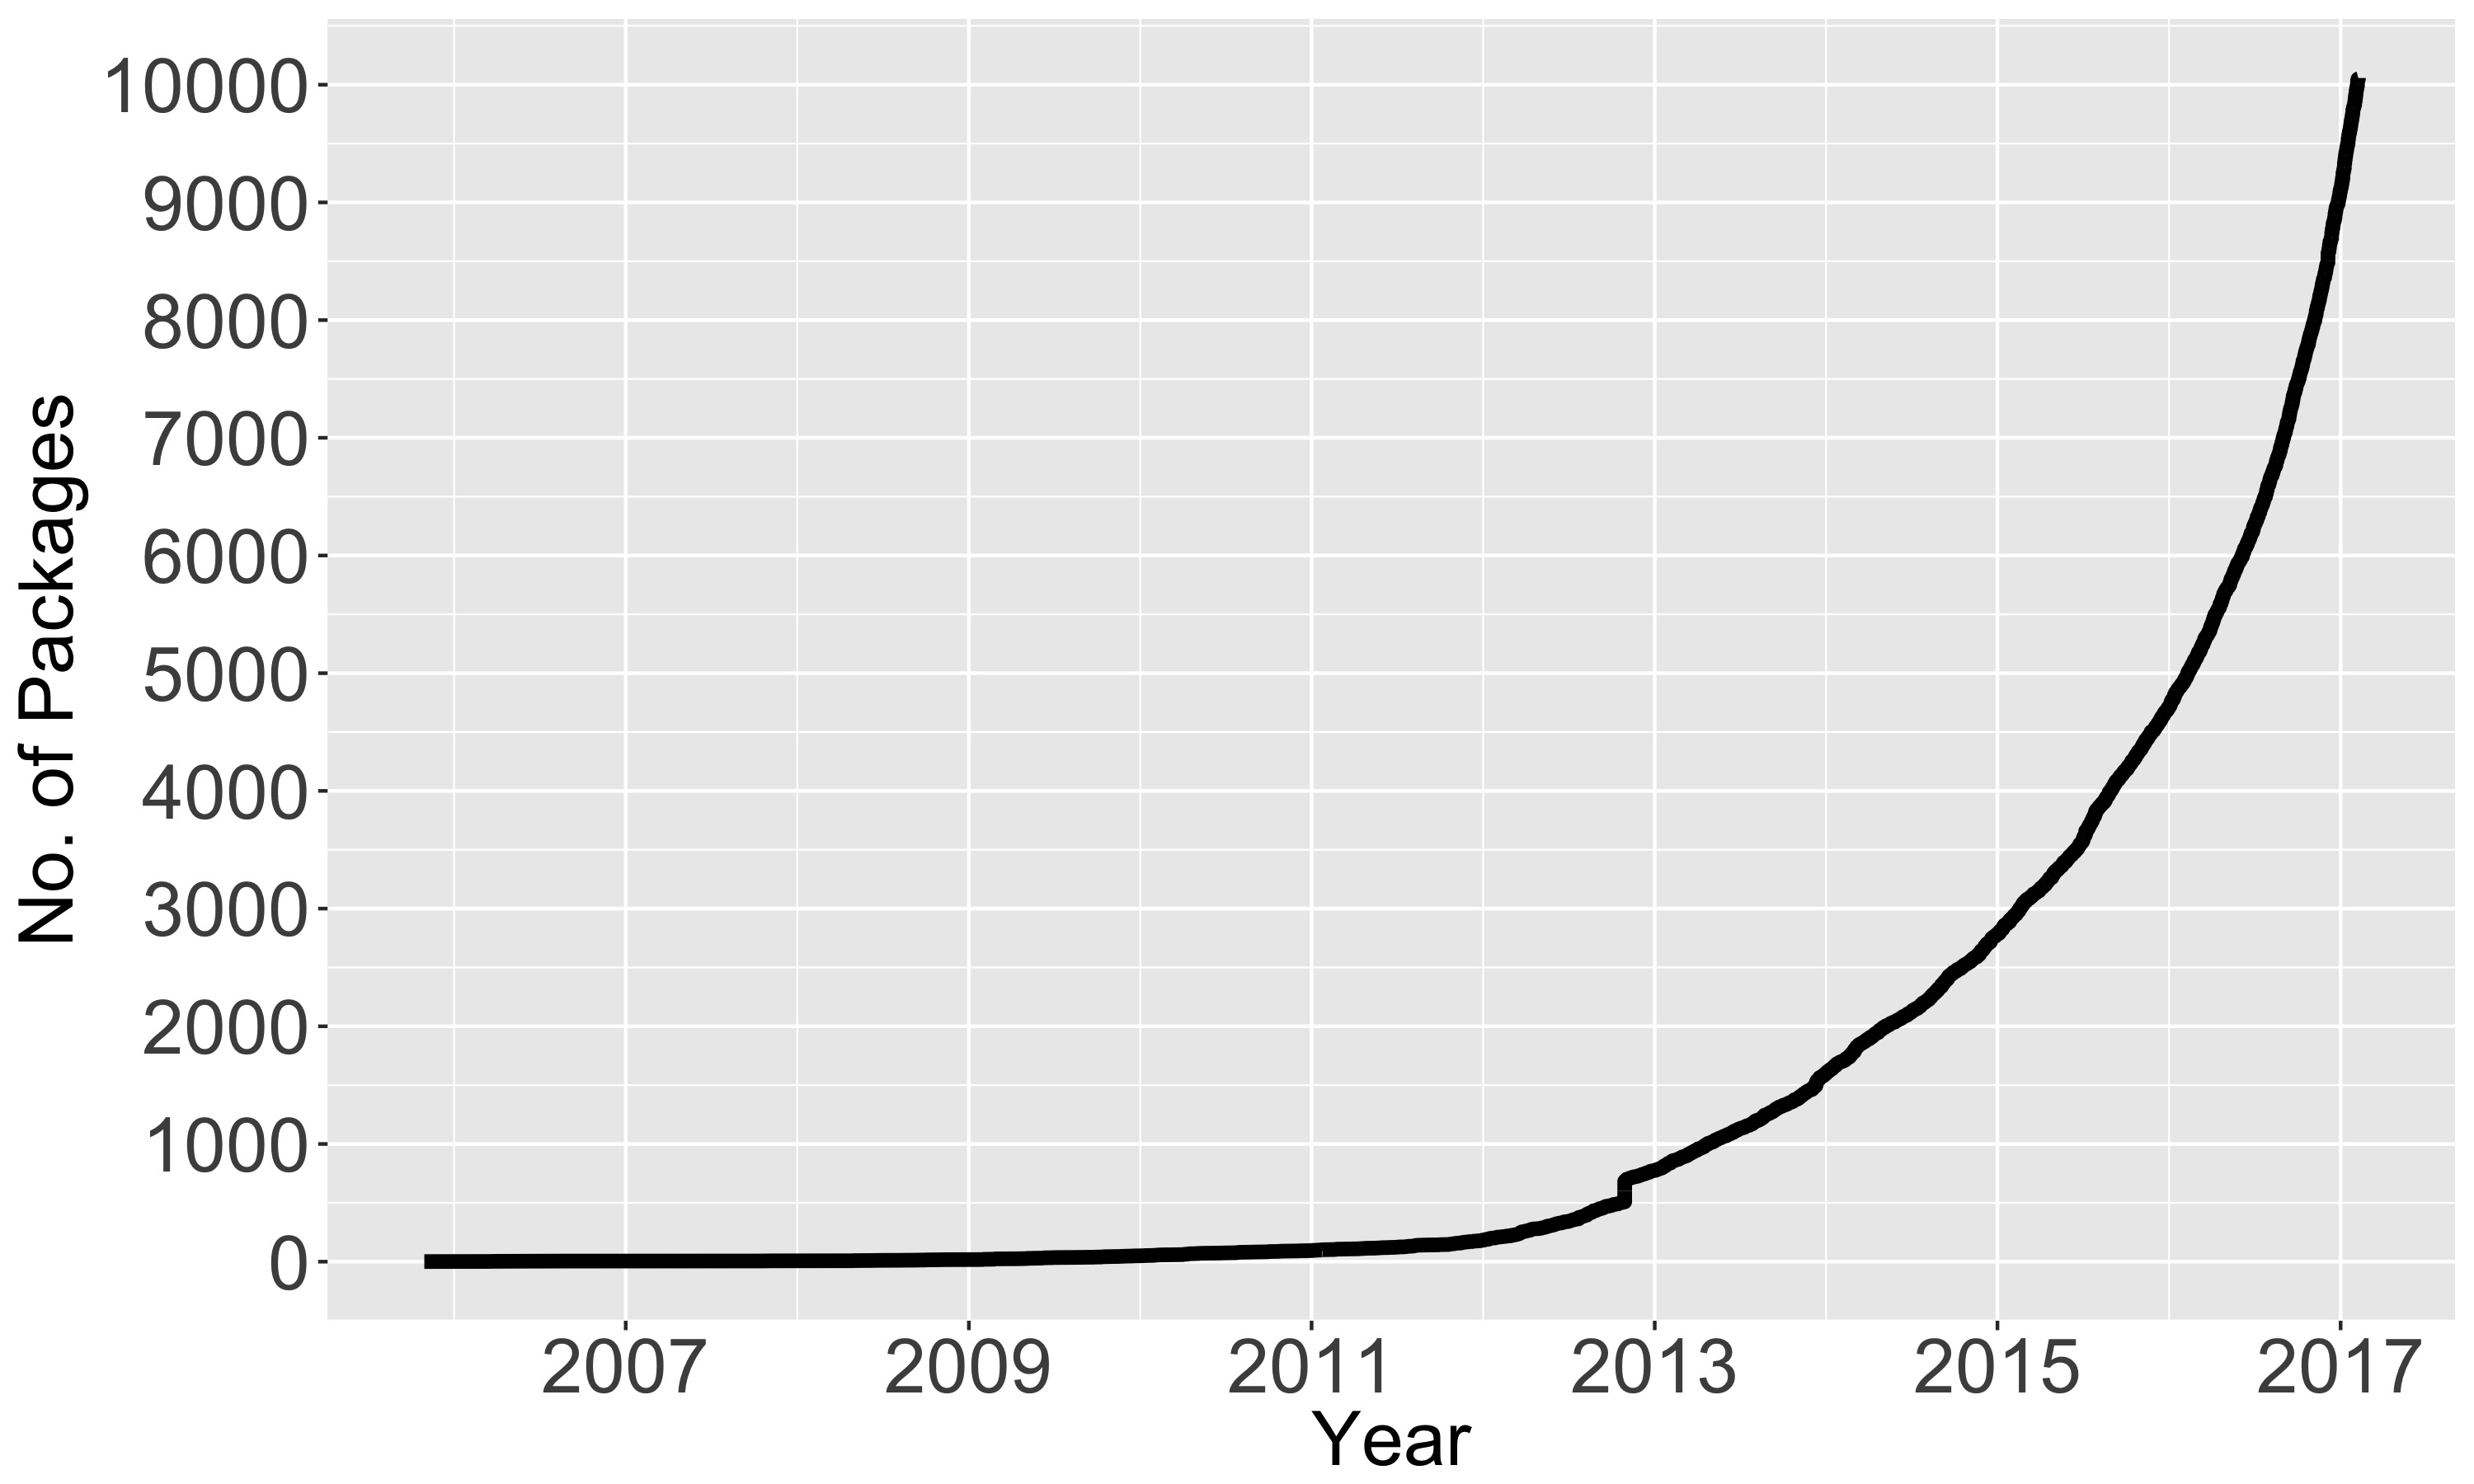
\includegraphics[scale = 0.1]{CRANpkgTrends.jpg}
\end{center}
\end{frame}

%%%%%

\begin{frame}{Reproducible Research with \texttt{R}}

  \begin{itemize}
    \item Automation of Workflow:
  \end{itemize}

\begin{center}
data $\rightarrow$ \underline{analysis code + explanatory text} $\rightarrow$ figures + tables + text = report
\end{center}

  \begin{itemize}
    \item Many resources for reproducible research
    \item Several possible input formats
    \item Typical output formats are pdf files and web pages
    \item This presentation written with \LaTeX \ and \texttt{R} via the knitr package.
  \end{itemize}
\end{frame}

%%%%%
\section*{ChemoSpec}

\begin{frame}{What is ChemoSpec?}
  \begin{itemize}
  \item ChemoSpec = Chemometrics + Spectroscopy
  \item Tools for exploratory data analysis
  \item No attempt to duplicate functions available on the spectrometer
  \end{itemize}
\end{frame}

%%%%%

\begin{frame}{ChemoSpec: Design Goals}
  \begin{itemize}
  \item User friendly design
  \item Helpful error messages
  \item Reliable results
  \item High quality plots
  \item Consistent plot appearance
  \item Provide access to a wide range of chemometric operations
  \item Extensibility
  \item Developed with metabolomics and IR, NMR \& Raman in mind
  \end{itemize}
\end{frame}

%%%%%

\begin{frame}{What Can ChemoSpec Do?}
\begin{multicols}{2}
  \begin{itemize}
    \item Data Cleaning \& Prep
      \begin{itemize}
        \item Import data
        \item Remove samples
        \item Drop frequency ranges
        \item Baseline correction
        \item Signal alignment
        \item Normalization
        \item Savitzky-Golay filters
      \end{itemize}
  \end{itemize}
\columnbreak
  \begin{itemize}
    \item Exploratory Data Analysis
      \begin{itemize}
        \item Plotting \& surveying
        \item Hierarchical cluster analysis (HCA)
        \item Principal component analysis (PCA)
        \item PCA diagnostics
        \item Score \& loading plots
        \item ANOVA-PCA
        \item Empirical clustering
      \end{itemize}
  \end{itemize}
\end{multicols}

\end{frame}

%%%%%
\section*{Demo}

\begin{frame}{Demonstration Data Set: Saw Palmetto Caps}
  \begin{itemize}
  \item Retail samples of \emph{Serenoa repens} gel caps
  \item 500 MHz \ce{^{1}H} NMR in \ce{CDCl3}
  \item 4 samples were pure according to the label
  \item 10 samples have another oil present per label
  \item 2 outliers: olive oil, and evening primrose oil
  \item \emph{Serenoa repens} extracts mainly fatty acids
  \item Outliers mainly triglycerides
  \end{itemize}
\end{frame}

%%%%%

\begin{frame}{Representative \ce{^{1}H} NMR Spectra}

\begin{knitrout}
\definecolor{shadecolor}{rgb}{0.969, 0.969, 0.969}\color{fgcolor}
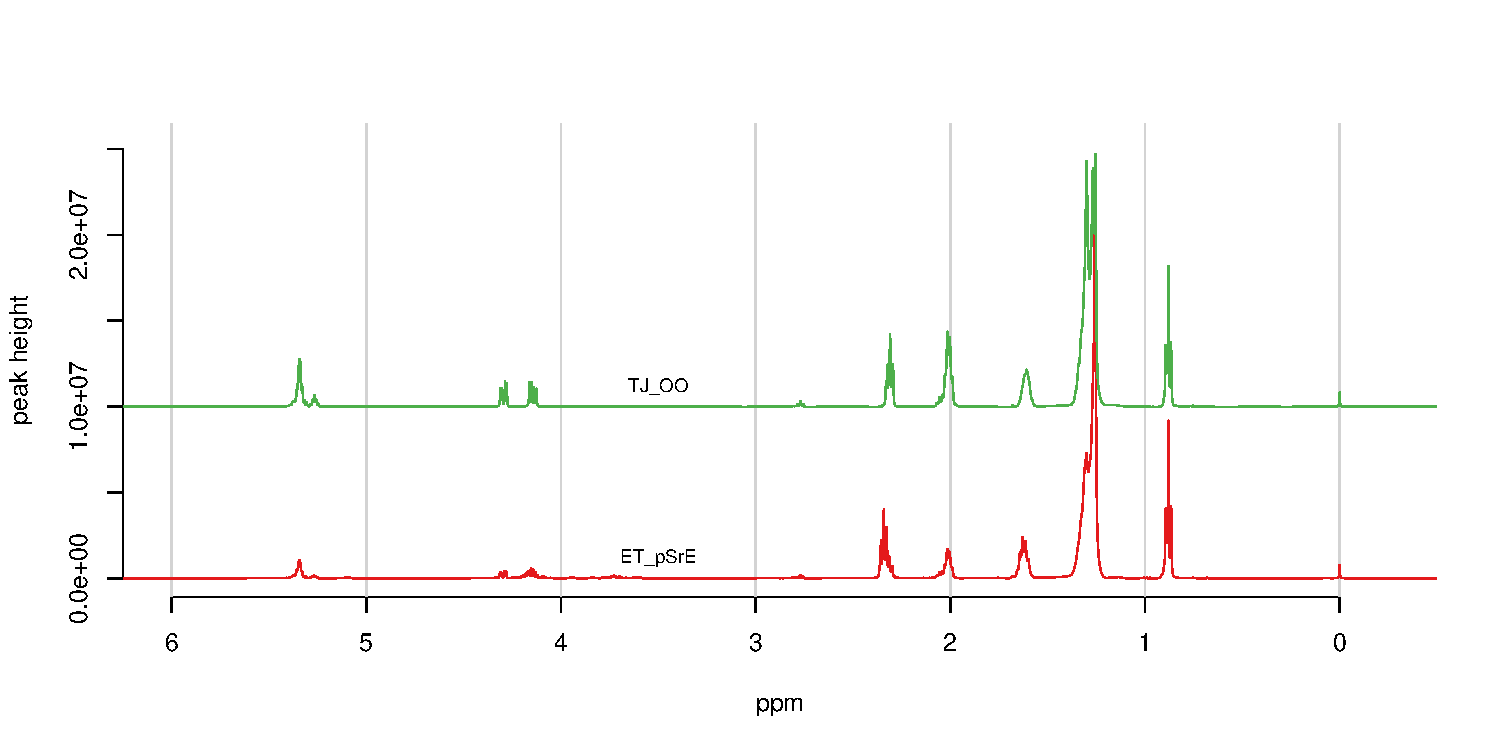
\includegraphics[width=\maxwidth]{figure/Spectra-1} 

\end{knitrout}

\end{frame}

%%%%%

\begin{frame}{Where is the Variation in the \ce{^{1}H} NMR Spectra?}

\begin{knitrout}
\definecolor{shadecolor}{rgb}{0.969, 0.969, 0.969}\color{fgcolor}
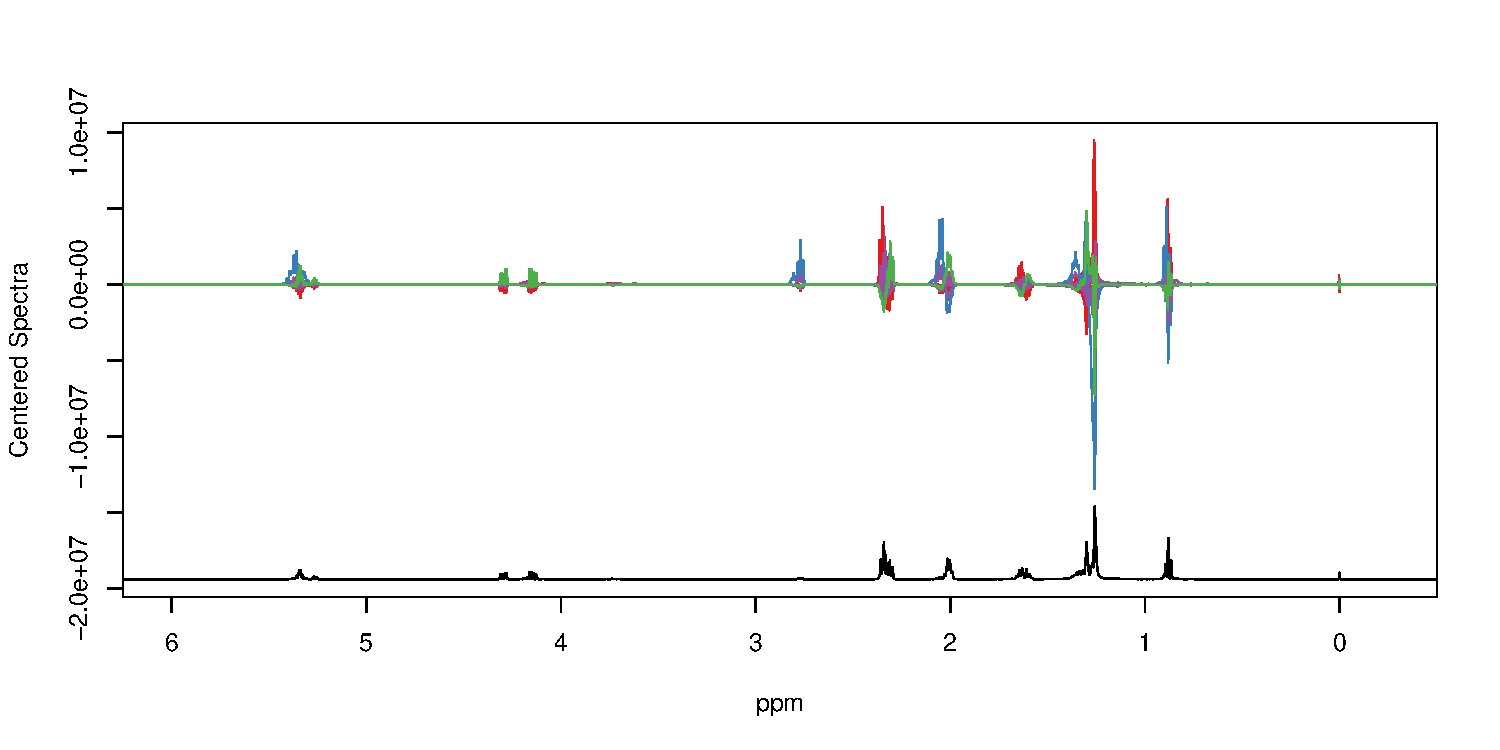
\includegraphics[width=\maxwidth]{figure/Survey-1} 

\end{knitrout}

\end{frame}

%%%%%

\begin{frame}{Hierarchical Clustering}

\begin{knitrout}
\definecolor{shadecolor}{rgb}{0.969, 0.969, 0.969}\color{fgcolor}
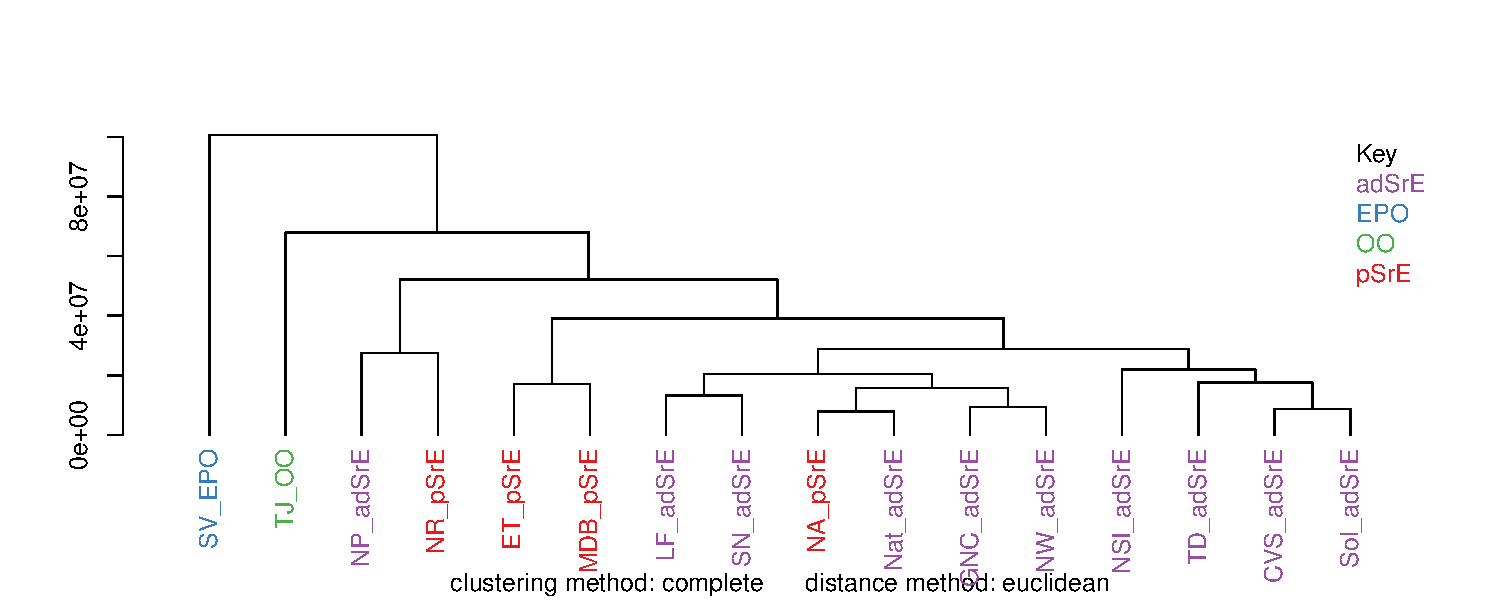
\includegraphics[width=\maxwidth]{figure/HCA-1} 

\end{knitrout}

\end{frame}

%%%%%

\begin{frame}{Principal Component Analysis: Scree Plot}

\begin{knitrout}
\definecolor{shadecolor}{rgb}{0.969, 0.969, 0.969}\color{fgcolor}
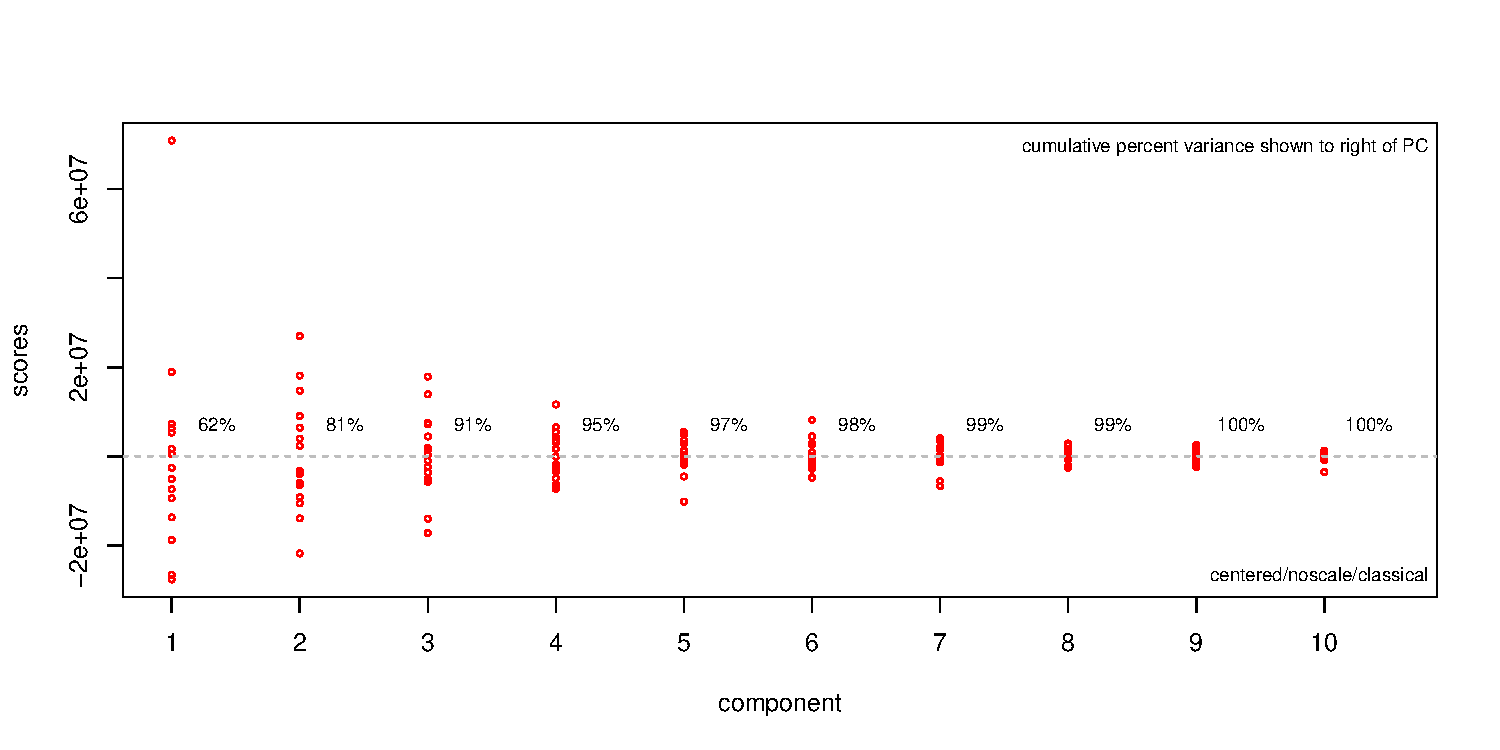
\includegraphics[width=\maxwidth]{figure/scree-1} 

\end{knitrout}

\end{frame}

%%%%%

\begin{frame}{Principal Component Analysis: Score Plot}

\begin{knitrout}
\definecolor{shadecolor}{rgb}{0.969, 0.969, 0.969}\color{fgcolor}
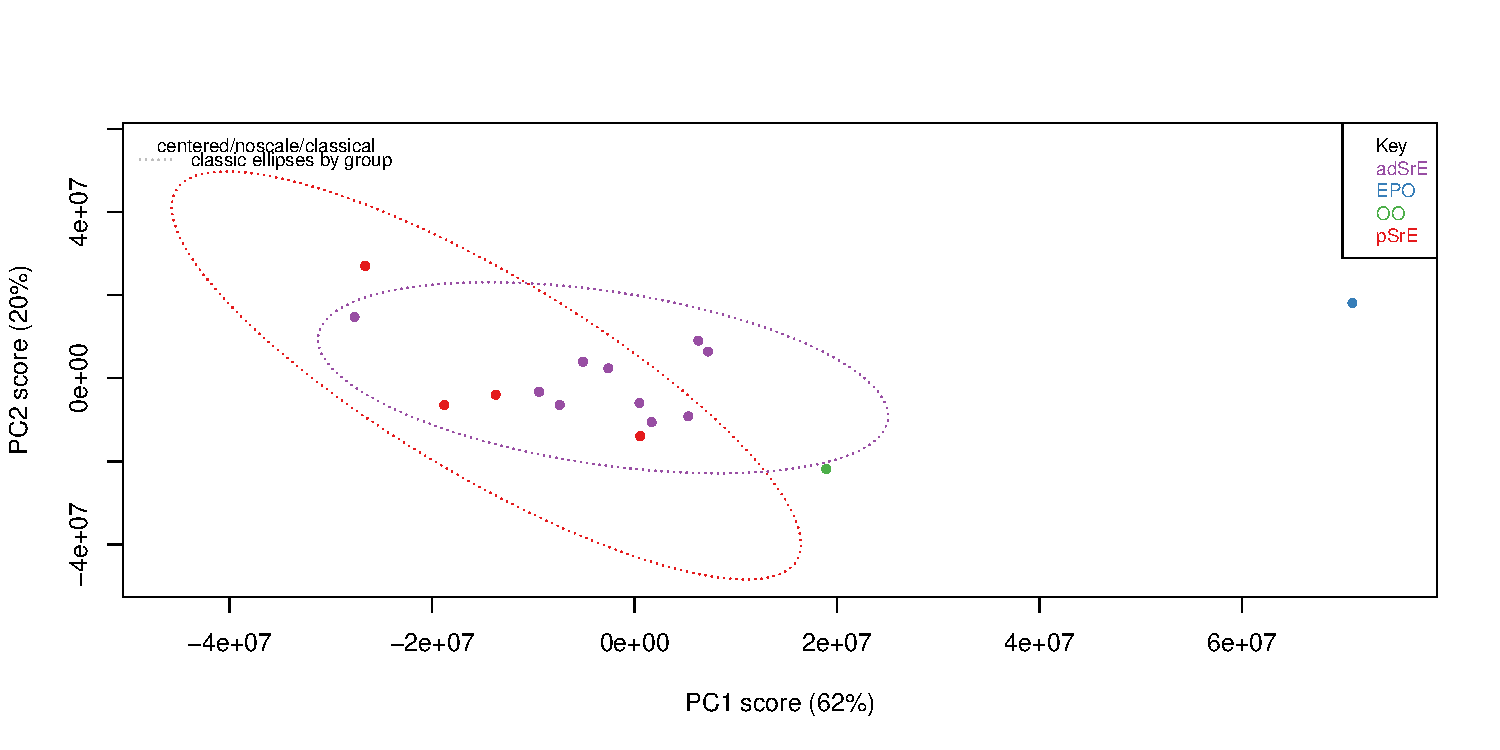
\includegraphics[width=\maxwidth]{figure/scores-1} 

\end{knitrout}

\end{frame}

%%%%%

\begin{frame}{Principal Component Analysis: Loadings Plot}

\begin{knitrout}
\definecolor{shadecolor}{rgb}{0.969, 0.969, 0.969}\color{fgcolor}
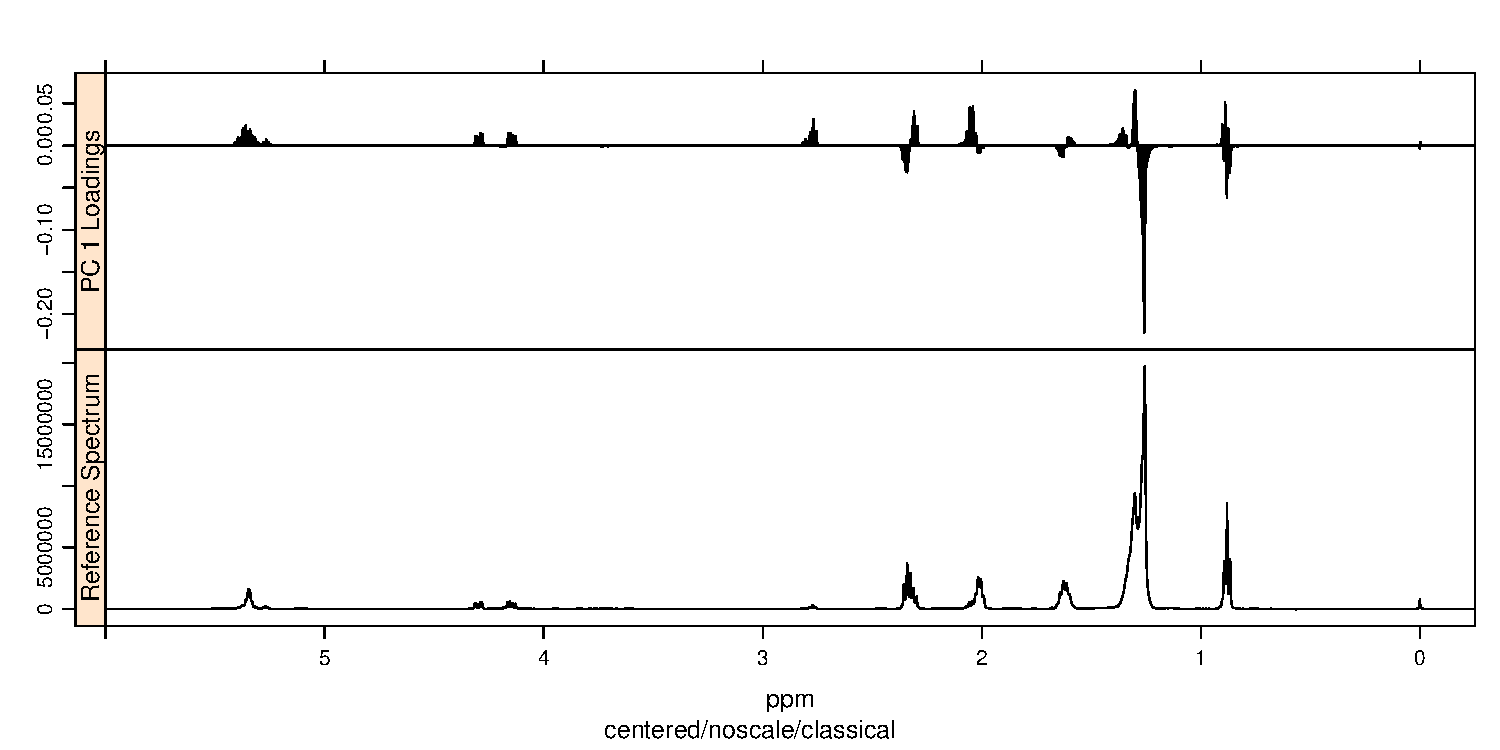
\includegraphics[width=\maxwidth]{figure/loadings-1} 

\end{knitrout}

\end{frame}

%%%%%

\begin{frame}{Principal Component Analysis: "S" Plot}

\begin{knitrout}
\definecolor{shadecolor}{rgb}{0.969, 0.969, 0.969}\color{fgcolor}
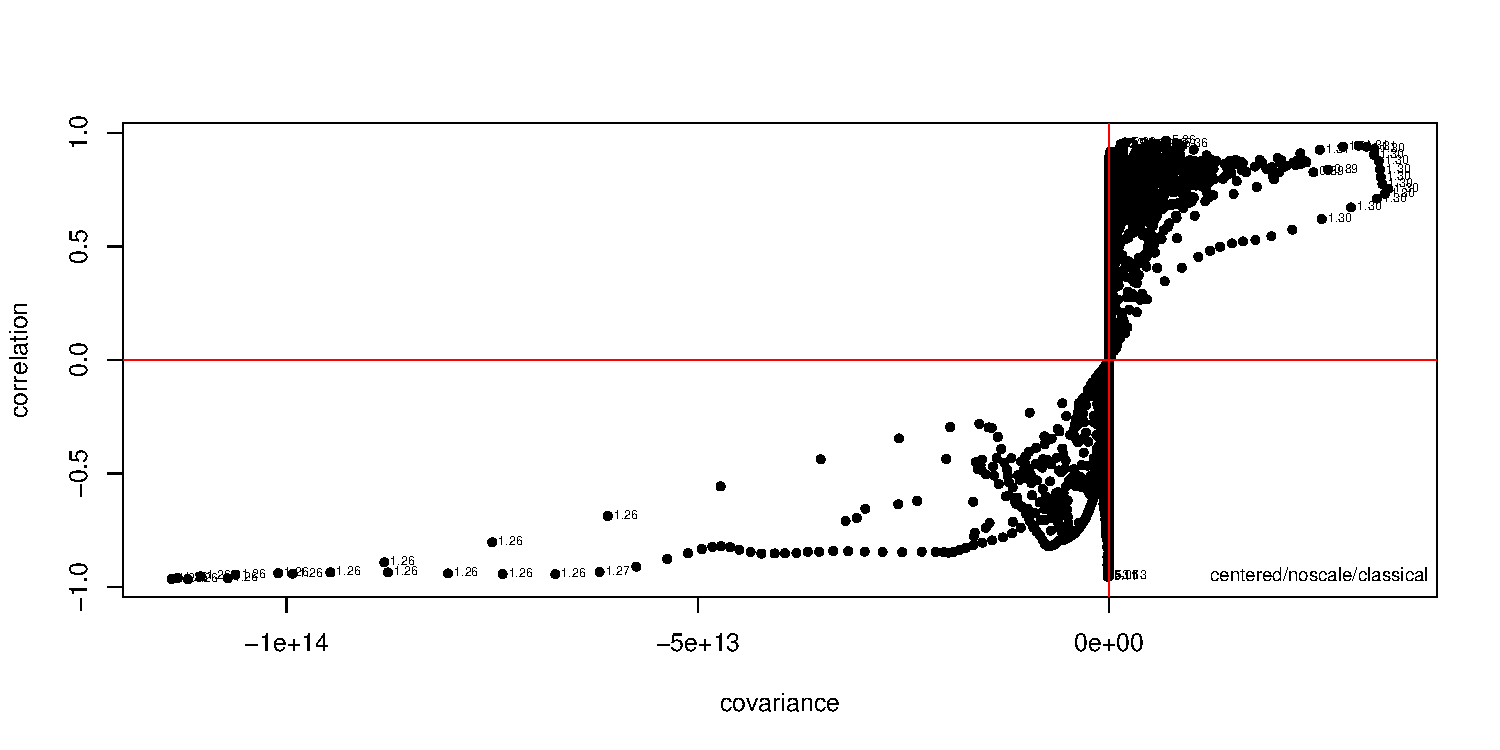
\includegraphics[width=\maxwidth]{figure/splot-1} 

\end{knitrout}

\end{frame}

\section*{The End}

%%%%%

\begin{frame}{Acknowledgements}
  \begin{itemize}
  \item Thanks for your attention!
  \item Kristie Adams for the invite
  \item Sabbatical Support, DePauw University
  \end{itemize}
\end{frame}

%%%%%

\begin{frame}{Additional References \& Resources}
  \begin{itemize}
    \item \href{https://www.r-project.org/}{\textcolor{red}{\texttt{R} Project Home Page}}
    \item  \href{https://cran.r-project.org/web/views/}{\textcolor{red}{Selected Topical Task Views}}
      \begin{itemize}
        \item \href{https://cran.r-project.org/web/views/ChemPhys.html}{\textcolor{red}{Chemometrics \& Computational Physics}}
        \item \href{https://cran.r-project.org/web/views/ClinicalTrials.html}{\textcolor{red}{Clinical Trials}}
        \item \href{https://cran.r-project.org/web/views/ExperimentalDesign.html}{\textcolor{red}{Experimental Design}}
        \item \href{https://cran.r-project.org/web/views/Pharmacokinetics.html}{\textcolor{red}{Pharmacokinetics}}
        \item \href{https://cran.r-project.org/web/views/MachineLearning.html}{\textcolor{red}{Machine Learning}}
        \item \href{https://cran.r-project.org/web/views/ReproducibleResearch.html}{\textcolor{red}{Reproducible Research}}
      \end{itemize}
    \item  \href{https://bioconductor.org/}{\textcolor{red}{Bioconductor Home Page}}
  \end{itemize}
\end{frame}


\end{document}
